\Chapter{Modélisation par les vitesses de dérive}
\chaptermark{Les vitesses de dérive}
Ce deuxième chapitre se concentre sur l'étude de la modélisation du transport
(fortement) magnétisé en contact avec une paroi. Nous présentons dans cet objectif 
le code TOKAM2D~\cite{Sarazin} utilisé pour
caractériser la SOL des tokamaks ainsi que les modifications qui lui ont été
apportées pour lui permettre décrire le transport dans des conditions se
rapprochant de notre étude.
Nous détaillerons enfin un modèle plasmas
froids/magnétisés basé sur les vitesses de dérive.
\section{Transport fortement magnétisé dans la SOL}
\chaptermark{Transport dans le plasma de bord}
La première partie de cette thèse a consisté à étudier et à modifier un modèle
fluide décrivant le transport magnétisé de la SOL des tokamaks.
\subsection{Le code TOKAM2D}
Le code TOKAM2D a été initialement développé à l'IMTM\footnote{Institut
Méditerranéen Technologique de Marseille} pour étudier la turbulence
d'interchange qui domine le transport transverse dans le plasma de bord des
tokamaks. Sa modification pour intégrer un forçage de la turbulence par un flux
au lieu d'un gradient d'équilibre a permis de retrouver le caractère
intermittent du transport et la longueur de décroissance du profil de densité
que l'on mesurait expérimentalement. L'étude du modèle a aussi amélioré la
compréhension du mécanisme principal de l'instabilité, dont le déclenchement à
seuil de l'interchange et la nature de type avalanche du transport turbulent.

C'est un code fluide, quasineutre, qui décrit le transport transverse en se
basant sur l'approximation des vitesses de dérive (voir §
\ref{Introduction}-\ref{vitessesDerive}).
\subsection{Hypothèses du modèle}
Dans les conditions typiques de la SOL, l'utilisation d'un modèle fluide est
justifiée par la forte collisionnalité du plasma. Le libre parcours moyen
$\lambda_{ei}=v_T \nu_{ei}$, de l'ordre du mètre, est très inférieur à la
longueur de connexion parallèle des lignes de champ $L_\para=2\pi q R\approx
$\unit{100}{\meter}.
Le plasma est de plus très magnétisé $B\approx$\unit{1}{\tesla}, les fréquences
caractéristiques du transport transverse sont donc très lentes devant la fréquence
cyclotronique ionique ce qui nous permet de nous placer dans le cadre de
l'approche des vitesse de dérives :
\begin{equation}
\omega\ll\omega_c\Leftrightarrow \varepsilon_\omega\equiv\frac{\omega}{\omega_c}\ll 1
\end{equation}

\begin{wrapfigure}{r}{0.50\textwidth}
	\vspace{-5pt}

 \hspace{20pt}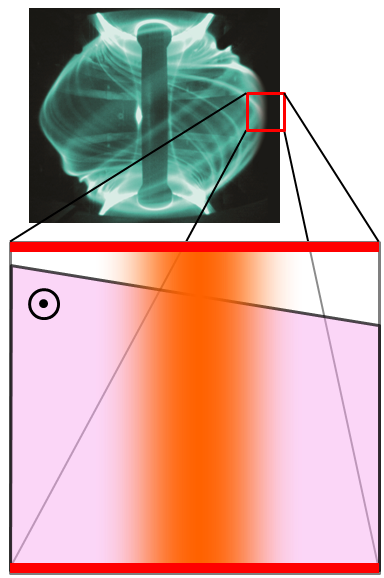
\includegraphics[width=0.40\textwidth]{figures/geomTokam.png}{\caption{Zone
de la SOL simulée dans TOKAM2D.}\label{figTokamGeom}}
	 \vspace{-20pt}
\end{wrapfigure}

D'un autre côté $\rho_L^i$, le rayon de Larmor ionique, d'environ
\unit{1}{\milli\meter}, est bien supérieur à la longueur de
Debye $\lambda_D$, de l'ordre de \unit{10^{-5}}{\meter}, ce qui permet de
considérer le plasma quasineutre dans son ensemble
, avec des densités ionique et électronique équales à $n$.

On décrit alors le transport du plasma à travers l'évolution de la densité
électronique $n_e=n$ et du potentiel électrostatique $U$ en résolvant l'équation
de continuité des électrons ainsi que l'équation de conservation du courant. Les
températures électronique
$T_e$ et ionique $T_i$ sont supposées constantes, avec un rapport $\tau=T_i/T_e$.

La zone simulée, présentée sur la figure~\ref{figTokamGeom}, correspond à  
L'hypothèse flûte, qui permet la réduction du problème de trois à deux
dimensions .
\subsection{Dérivation des équations}
\subsubsection{Equation de conservation de la matière}
En notant $D_\perp$ le coefficient de diffusion rendant compte des collisions,
et $S$ un terme source pour modéliser le flux de particules provenant du plasma
de coeur, l'équation de continuité des électrons s'écrit :
\begin{equation}
\label{2-ContinuiteElectrons}
\partial_t n + \nabla\cdot(n\mathbf{u}^e) = D_\perp\nabla^2_\perp n + S
\end{equation}

Comme discuté dans le chapitre précédent, le flux de matière transverse est
essentiellement issu de l'advection par la vitesse de
dérive électrique. L'équation \ref{2-ContinuiteElectrons} se transforme donc en :
\begin{equation}
\label{2-ContinuiteElectrons2}
\partial_t n + \nabla_\para\cdot(n\mathbf{u}^e_{\para}) =
\mathbf{u}_E\cdot\nabla_\perp n + D_\perp\nabla^2_\perp n + S
\end{equation}

Le terme d'advection $\mathbf{u}_E\cdot\nabla_\perp
n$ peut se réécrire en utilisant la notation
du crochet de Poisson $[n,U]=\mathbf{b}.(\nabla_\perp n\times\nabla_\perp U)$.
C'est la forme que prend toute advection d'un champ scalaire par une vitesse de
dérive $\mathbf{v}^\text{d}=\nabla H\times\mathbf{B}/B^2$, où $\nabla H$ est la
force à l'origine de la dérive. L'équation de continuité pour les électrons est
alors :
\begin{equation}
\partial_t n + \nabla_{\para}\cdot(n\mathbf{u}^e_{\para}) =
\frac{1}{B}\left[n,U\right] + D_\perp\nabla^2_\perp n + S
\end{equation}

Le terme non-linéraire $[n,U]$ est l'un des éléments moteur du modèle
d'interchange, couplant la densité au potentiel électrique, il opère un
transfert d'exitation des composantes radiales des fluctuations à leurs
composantes poloïdales et réciproquement. Les termes de flux parallèle et de
diffusion sont stabilisant, ils tendent à
amortir les fluctuations et donc à homogénéiser le système.

\subsubsection{Equation de conservation du courant}
L'équation de conservation du courant s'obtient en soustrayant l'équation de
continuité des électrons à celle des ions. La vitesse de dérive électrique
$\mathbf{u}^E$, indépendante de la masse et de la charge des particules, est
identique pour les deux espèces et ne transporte donc aucun courant. 
La conservation du courant se résume ainsi à un équilibre entre le courant
parallèle et les courants transverses diamagnétique et de polarisation à
travers leur divergences:
\begin{equation}
\label{EqCourant1}
\nabla\cdot\left(\mathbf{j}\right) = 
\nabla\cdot\left(\mathbf{j}_\para+\mathbf{j}_*+\mathbf{j}_p\right)
= 0
\end{equation}

La divergence du courant diamagnétique donne un crochet de Poisson :
\begin{equation}
\nabla_\perp\cdot\mathbf{j}_*=
\nabla_\perp\cdot\left(\nabla_\perp\left(
P_i+P_e\right)\times\mathbf{B}/B^2\right) = \left[P_i+P_e,B\puissance{-1}\right]
\end{equation}

La vitesse de polarisation étant proportionnelle à la masse des particules
(Eq.~\ref{Introduction}-\ref{vitessesDerive}), on ne retient dans l'expression
du courant que la contribution ionique
$\mathbf{j}_p\approx\text{e}n\mathbf{u}^i_p$. En prenant en compte une viscosité
$\nu_\perp$, la dérivée totale est approximée par :
\begin{equation}
\frac{\text{d}\nabla_\perp U}{\text{dt}} \equiv 
\left(\partial_\text{t} - \nu_\perp \nabla_\perp^2 +
\mathbf{u}^i\cdot\nabla_\perp\right)\nabla_\perp U
\end{equation}

De manière similaire à Eq.~\ref{2-ContinuiteElectrons2}, seule l'advection par
la vitesse de dérive électrique est considérée dans la divergence.
Eq.~\ref{EqCourant1} se réécrit alors :
\begin{equation}\begin{split}
\label{EqCourant2}
\nabla_\para\cdot\mathbf{j}_\para + \left[P_i+P_e,B\puissance{-1}\right] +
\nabla_\perp\cdot\left(-\frac{n\text{m}_i}{B^2}\left(\partial_\text{t}\nabla_\perp
U - \nu_\perp \nabla_\perp^3 U \right)\right) \\+
\nabla_\perp\cdot\left(-\frac{nm_\text{i}}{B^2}\mathbf{u}_E\cdot\nabla_\perp^2
U\right)=0
\end{split}
\end{equation}

Diverses considérations sur l'importance relative des termes contenus dans
Eq.~\ref{EqCourant2} (reliées entre autres aux hypothèses d'ordering ou aux
variations et à la finitude du rayon de Larmor) sont développées dans
\cite{Sarazin} pour simplifier le modèle. Elles conduisent à l'expression
finale de l'équation du courant :
\begin{equation}\begin{split}
\label{EqCourantFinale}
\nabla_\para\cdot\mathbf{j}_\para +
(T_e+T_i)\left[n,B\puissance{-1}\right] =\\
\frac{nm_i}{B^2}\left(\partial_\text{t}\nabla_\perp^2 U - \nu_\perp
\nabla_\perp^4U+
B\puissance{-1}\left[U,\nabla_\perp^2\ U\right]\right)
\end{split}
\end{equation}


\subsection{Normalisation du système}
Les grandeurs de normalisation sont reliées à l'intensité du champ magnétique
$B\indice{0}$ et à la température électronique de référence $T\indice{0}$. Le
temps est normalisé à l'inverse de la fréquence cyclotronique ionique :
\begin{equation}
t = \overline{t}\:\omega_c\puissance{-1} =
\overline{t}\:\frac{m_i}{eB\indice{0}}
\end{equation}
Les longueurs et vitesses sont alors logiquement normalisées par le rayon de
Larmor et la vitesse de Bohm :

\begin{eqnarray}
x = \overline{x}\:\rho_L =
\overline{x}\:\frac{m_ic_s}{eB\indice{0}} &
et &
v=\overline{v}\:c_s=\overline{v}\left(\frac{eT\indice{0}}{m_i}\right)^{\text{\textonehalf}}
\end{eqnarray}

Nous définissons de plus les variables adimensionnées du modèle, la densité
$\overline{N}$ et le potentiel électrostatique $\overline \phi$ par :
\begin{eqnarray}
n = n_{\indice{0}}\:\overline{N} & \text{et} & U=\frac{\overline
{\phi}T\indice{0}}{e}
\end{eqnarray}
\vfill
\section{Vers une description des sources d'ions}
L'approche par les vitesses de dérive utilisée pour construire le modèle de TOKAM2D n'est pas 
réellement justifiée dans le cas des sources d'ions. Le modèle suppose tout d'abord une
forte magnétisation des particules, $v_\perp<<v_\text{th}$, ce qui n'est pas du tout le cas dans 
les zones faiblement ou non-magnétisées. Les équations de TOKAM2D ne décrivent pas non plus l'intéraction
collisionnelle des particules chargées avec la population neutre, essentielle dans la physique des plasmas froids,
(ceci pouvant éventuellement être modifié, cf.
partie~\ref{vitessesDerivePlasmaFroid}).

Le code TOKAM2D peut toutefois être complété pour décrire des cas limites de notre étude, \emph{ie.} des plasmas totalement ionisés
confinés par un champ magnétique suffisement intense. Les questions de confinement transverse, d'inhomogénéité du champ 
magnétique et d'influence de la température sont alors utiles pour :
\begin{itemize}
	\item mesurer les approximations faites dans TOKAM2D et leur impact sur le transport transverse dans la SOL
	\item donner un aperçu du transport dans des configurations de type source d'ions, ainsi que des résultats sur les 
	cas limites fortement magnétisés à étudier et comparer.
\end{itemize}
	\subsection{Ajout des conditions aux limites transverses}
	Les systèmes physiques décrits par les équations fluides sont très sensibles aux conditions limites. Ces conditions étant 
	souvent mal connues, on peut les choisir de facon arbitraire, mais avec quel impact sur le système? La simplification de 
	TOKAM2D de considérer une géométrie bipériodique dans le plan transverse est fondamentalement injustifiée, mais a-t-elle une 
	influence sur le transport transverse en soi? Quels sont les effets d'autres conditions aux limites courament utilisées? 
	
	La prise en compte de conditions aux limites physiques telle que des conditions dérivées du critère de Bohm 
	sont nécéssaires pour décrire correctement la physique du transport dans les plasmas. Cependant bien que la théorie des
	gaines prédise le même comportement dans le cas des plasmas froids et que dans celui des plasmas magnétisés le long des lignes de 
	champ, la situation d'une gaine parallèle au champ magnétique est très mal connue dans la littérature.
	
	\subsection{Inclusion d'un champ magnétique non uniforme}
	Dans les plasmas de fusions, l'inhomogénéité du champ magnétique est responsable d'une majeure partie du transport turbulent.
	L'inclusion d'un champ magnétique inhomogène en espace a permis d'élargir le domaine de fonctionnalité de TOKAM2D. 
	
	Le cas d'une barrière magnétique montre...
	De très faibles inhomogénéités pouvant être responsable d'une modification non-négligeable du transport transverse, il pourrait 
	être intéressant de poursuivre l'étude dans cette direction.
	
	\subsection{Implémentation de l'équation d'énergie}
	La fermeture isoterme considérée dans le modèle de TOKAM2D est aussi très discutable. Les effets de la température et de la chaleur
	deviennent non-négligeables dès que $\omega>>\text{?}$. De plus la prise en compte des variations spatiales de la température
	complexifie grandement la relation de dispersion du modèle, et pouvant donner lieu à l'apparition d'instabilités différentes de 
	l'interchange.
	Les équations du modèle s'écrivent alors :
	
	\begin{equation}\begin{split}
		\partial_t N + \nabla_\perp\cdot\left(NB^{^{-2}}\mathbf{E}\times\mathbf{B}\right)
		+ \nabla_\perp\cdot\left(B^{^{-2}}\nabla P_e\times\mathbf{B}\right)
		  \\= \sigma_\para N{T_e}^{\text{\textonehalf}} exp({\Lambda-\Delta\Phi/T_e}) 
		 + D_\perp\nabla^2_\perp N + S
		 \end{split}
	\end{equation}
	
	aa
	
	\begin{equation}\begin{split}
			\partial_\text{t}\nabla_\perp^2 \Phi +\nabla_\perp\cdot\left(\nabla_\perp^2 \Phi\frac{\mathbf{E}\times\mathbf{B}}{B^2}\right)
			+ \nabla_\perp\cdot\left(\frac{\nabla P\times\mathbf{B}}{B^2}\right)
			\\= 
		\sigma_\para {T_e}^{\text{\textonehalf}}\left(1-e^{\Lambda-\Delta\Phi/T_e}\right) +\nu_\perp\nabla_\perp^4\Phi
	\end{split}\end{equation}
	
	aa
	
\section{Application de l'approche par vitesse de dérive pour les plasmas
froids}
\label{vitessesDerivePlasmaFroid}
Dans les plasmas froids,

\bibliographystyle{alpha}
\bibliography{biblio}





